\chapter{Transforming Functions}

Let's say I gave you the graph of a function $f$, like this:

\begin{tikzpicture}
    \begin{axis}[
        xmin=-2.2,xmax=2.2,
        ymin=-1,ymax=5,
        axis x line=middle,
        axis y line=middle,
        axis line style=<->,
        xlabel={$x$},
        ylabel={$y$},
      ]
      \addplot[no marks,sdkblue] expression[domain=-2:2,samples=100]{x^2} node[below, yshift=-6mm] {$f(x)$};
    \end{axis}\end{tikzpicture}

And then I tell you that the function $g(x) = f(x) + 1.5$.  Can you guess what the graph of $g$ would look like? It is the same graph, just translated up 1.5:

\begin{tikzpicture}
    \begin{axis}[
        xmin=-2.2,xmax=2.2,
        ymin=-1,ymax=5,
        axis x line=middle,
        axis y line=middle,
        axis line style=<->,
        xlabel={$x$},
        ylabel={$y$},
      ]
      \addplot[dashed,sdkblue] expression[domain=-2:2,samples=100]{x^2} node[below, yshift=-6mm] {$f(x)$};
      \addplot[no marks,sdkblue] expression[domain=-2:2,samples=100]{x^2 + 1.5} node[below, yshift=-6mm] {$g(x)$};
    \end{axis}\end{tikzpicture}

There are four kinds of transformations that we do all the time:
\begin{itemize}
\item Translation up and down in the direction of $y$ axis (the one you just saw)
\item Translation left and right in the direction of the $x$ axis
\item Scaling up and down along the $y$ axis
\item Scaling up and down along the $x$ axis
\end{itemize}

Now I will demonstrate each of the four using the graph of $\sin(x)$.

\section{Translation up and down}

When you add a positive constant to a function, you translate the
whole graph up that much. A negative constant translates it down.

Here is the graph of $\sin(x) - 0.5$:

\begin{tikzpicture}[
tl/.style = {% tick labels
    fill=white, inner sep=1pt, font=\scriptsize,
            },                        ]
% grid
\draw[sdkblue, very thin, xstep=0.5235, ystep=0.5] (-6.6,-1.7) grid (6.6,1.2);

% y tick label
\foreach \y in {-1, -1/2, 1/2, 1}{\node[tl,left=1mm] at (0,\y) {$\y$};}
% x tick label
\foreach \x [count=\xx from -4] in 
       {-2\pi,
        -\frac{3\pi}{2},
        -\pi,           
        -\frac{\pi}{2}, 
        { },
         \frac{\pi}{2},
         \pi, 
         \frac{3\pi}{2}, 
         2\pi
        }{\node[tl,below=1mm] at (3*0.5235*\xx,0) {$\x$};}
% axes
    \draw[->,thick] (-6.5,0) -- (6.5,0) node[right] {$x$};
    \draw[->,thick] (0,-1.25) -- (0, 1.25) node[above] {$y$};
% curve
\draw[<->,dashed,draw=black,
      domain=-6.5:6.5,samples=300,variable=\x] 
      plot (\x,{sin(deg{\x})});
\draw[<->,thick,draw=black,
      domain=-6.5:6.5,samples=300,variable=\x] 
      plot (\x,{sin(deg{\x}) - 0.5});
\end{tikzpicture}

\section{Translation left and right}

When you add a positive number to $x$ before running it through $f$,
you translate the graph to the left that much. Adding a negative
number translates the graph to the right.

Here is the graph of $\sin(x - \pi/6)$:

\begin{tikzpicture}[
tl/.style = {% tick labels
    fill=white, inner sep=1pt, font=\scriptsize,
            },                        ]
% grid
\draw[sdkblue, very thin, xstep=0.5236, ystep=0.5] (-6.6,-1.2) grid (6.6,1.2);

% y tick label
\foreach \y in {-1, -1/2, 1/2, 1}{\node[tl,left=1mm] at (0,\y) {$\y$};}
% x tick label
\foreach \x [count=\xx from -4] in 
       {-2\pi,
        -\frac{3\pi}{2},
        -\pi,           
        -\frac{\pi}{2}, 
        { },
         \frac{\pi}{2},
         \pi, 
         \frac{3\pi}{2}, 
         2\pi
        }{\node[tl,below=1mm] at (3*0.5235*\xx,0) {$\x$};}
% axes
    \draw[->,thick] (-6.5,0) -- (6.5,0) node[right] {$x$};
    \draw[->,thick] (0,-1.25) -- (0, 1.25) node[above] {$y$};
% curve
\draw[<->,dashed,draw=black,
      domain=-6.5:6.5,samples=300,variable=\x] 
      plot (\x,{sin(deg{\x})});
\draw[<->,thick,draw=black,
      domain=-6.5:6.5,samples=300,variable=\x] 
      plot (\x,{sin(deg{\x} - 30)});
\end{tikzpicture}

Notice the sign:
\begin{itemize}
\item Add to $x$ before processing with the function translates the graph to the \emph{left}.
\item Subtract from $x$ before processing with the function translates the graph to the \emph{right}
\end{itemize}

\section{Scaling up and down in the $y$ direction}

To scale the function up and down, you multiply the result of the
function by a constant.  If the constant is larger than 1, it
stretches the function up and down.

Here is $y = 2\sin(x)$:

\begin{tikzpicture}[
tl/.style = {% tick labels
    fill=white, inner sep=1pt, font=\scriptsize,
            },                        ]
% grid
\draw[sdkblue, very thin, xstep=0.5236, ystep=0.5] (-6.6,-2.2) grid (6.6,2.2);

% y tick label
\foreach \y in {-1, -1/2, 1/2, 1}{\node[tl,left=1mm] at (0,\y) {$\y$};}
% x tick label
\foreach \x [count=\xx from -4] in 
       {-2\pi,
        -\frac{3\pi}{2},
        -\pi,           
        -\frac{\pi}{2}, 
        { },
         \frac{\pi}{2},
         \pi, 
         \frac{3\pi}{2}, 
         2\pi
        }{\node[tl,below=1mm] at (3*0.5235*\xx,0) {$\x$};}
% axes
    \draw[->,thick] (-6.5,0) -- (6.5,0) node[right] {$x$};
    \draw[->,thick] (0,-1.25) -- (0, 1.25) node[above] {$y$};
% curve
\draw[<->,dashed,draw=black,
      domain=-6.5:6.5,samples=300,variable=\x] 
      plot (\x,{sin(deg{\x})});
\draw[<->,thick,draw=black,
      domain=-6.5:6.5,samples=300,variable=\x] 
      plot (\x,{sin(deg{\x}) * 2.0});
\end{tikzpicture}

With a wave like this, we speak of its \newterm{Amplitude}, which you
can think of as its height. The baseline that this wave oscillates
around is zero. The maximum distance that it gets from that baseline
is its amplitude.  Thus, the amplitude here has been increased from 1
to 2.

If you multiply by a negative number, the function gets flipped.  Here is $y = -0.5 \sin(x)$

\begin{tikzpicture}[
tl/.style = {% tick labels
    fill=white, inner sep=1pt, font=\scriptsize,
            },                        ]
% grid
\draw[sdkblue, very thin, xstep=0.5236, ystep=0.5] (-6.6,-1.2) grid (6.6,1.2);

% y tick label
\foreach \y in {-1, -1/2, 1/2, 1}{\node[tl,left=1mm] at (0,\y) {$\y$};}
% x tick label
\foreach \x [count=\xx from -4] in 
       {-2\pi,
        -\frac{3\pi}{2},
        -\pi,           
        -\frac{\pi}{2}, 
        { },
         \frac{\pi}{2},
         \pi, 
         \frac{3\pi}{2}, 
         2\pi
        }{\node[tl,below=1mm] at (3*0.5235*\xx,0) {$\x$};}
% axes
    \draw[->,thick] (-6.5,0) -- (6.5,0) node[right] {$x$};
    \draw[->,thick] (0,-1.25) -- (0, 1.25) node[above] {$y$};
% curve
\draw[<->,dashed,draw=black,
      domain=-6.5:6.5,samples=300,variable=\x] 
      plot (\x,{sin(deg{\x})});
\draw[<->,thick,draw=black,
      domain=-6.5:6.5,samples=300,variable=\x] 
      plot (\x,{sin(deg{\x}) * -0.5});
\end{tikzpicture}

Amplitude is never negative.  Thus, the amplitude of this wave is 0.5.

\section{Scaling up and down in the $x$ direction}

If you multiply $x$ by a number larger than 1 before running it
through the function, the graph gets compressed toward zero.

Here is $y = \sin(3x)$:

\begin{tikzpicture}[
tl/.style = {% tick labels
    fill=white, inner sep=1pt, font=\scriptsize,
            },                        ]
% grid
\draw[sdkblue, very thin, xstep=0.5236, ystep=0.5] (-6.6,-1.2) grid (6.6,1.2);

% y tick label
\foreach \y in {-1, -1/2, 1/2, 1}{\node[tl,left=1mm] at (0,\y) {$\y$};}
% x tick label
\foreach \x [count=\xx from -4] in 
       {-2\pi,
        -\frac{3\pi}{2},
        -\pi,           
        -\frac{\pi}{2}, 
        { },
         \frac{\pi}{2},
         \pi, 
         \frac{3\pi}{2}, 
         2\pi
        }{\node[tl,below=1mm] at (3*0.5235*\xx,0) {$\x$};}
% axes
    \draw[->,thick] (-6.5,0) -- (6.5,0) node[right] {$x$};
    \draw[->,thick] (0,-1.25) -- (0, 1.25) node[above] {$y$};
% curve
\draw[<->,dashed,draw=black,
      domain=-6.5:6.5,samples=300,variable=\x] 
      plot (\x,{sin(deg{\x})});
\draw[<->,thick,draw=black,
      domain=-6.5:6.5,samples=300,variable=\x] 
      plot (\x,{sin(deg{\x} * 3)});
\end{tikzpicture}

The distance between two peaks of a wave is known as its
\newterm{wavelength}.  The original wave had a wavelength of $2\pi$.
The compressed wave has a wavelength of $2\pi/3$.

If you multiply $x$ by a number smaller than 1, it will stretch the function out, away from the $y$ axis.

If you multiply $x$ by a negative number, it will flip the function around the $y$ axis.

Here is $y = 2^{(-0.5x)}$. Notice that it has flipped around the $y$ axis and is stretched out along the $x$ axis.

\begin{tikzpicture}
    \begin{axis}[
        xmin=-3.1,xmax=3.1,
        ymin=-0.5,ymax=8,
        axis x line=middle,
        axis y line=middle,
        axis line style=<->,
        xlabel={$x$},
        ylabel={$y$},
      ]
      \addplot[dashed,sdkblue] expression[domain=-3.0:3.0,samples=100]{2^x} node[left, xshift=-1mm,yshift=-6mm] {$2^x$};
      \addplot[no marks,sdkblue] expression[domain=-3.0:3.0,samples=100]{2^(-0.5 * x)}
      node[above, xshift=-6mm] {$2^{-0.5x}$};
    \end{axis}\end{tikzpicture}
    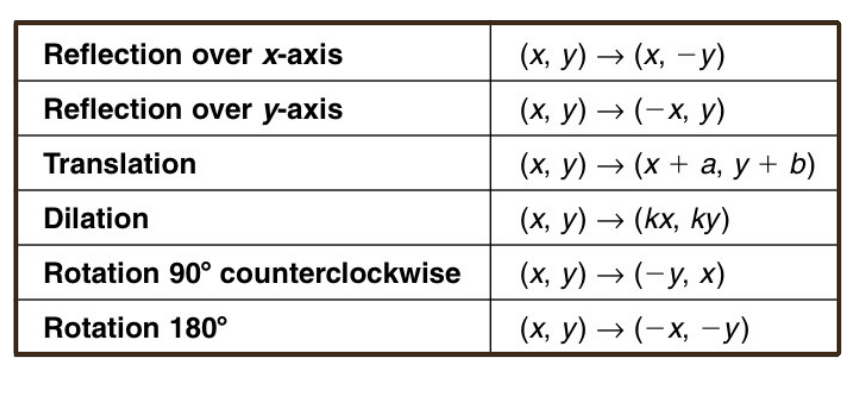
\includegraphics[width=0.8\textwidth]{transformation_r.png}

\section{Order is important!}

We can combine these transformations. This allows us, for example, to
translate a function up 2 and then scale along the $y$ axis by 3.

Here is $y = 2.0 (\sin(x) + 1)$:

\begin{tikzpicture}[
tl/.style = {% tick labels
    fill=white, inner sep=1pt, font=\scriptsize,
            },                        ]
% grid
\draw[sdkblue, very thin, xstep=0.5236, ystep=0.5] (-6.6,-1.2) grid (6.6,4.2);

% y tick label
\foreach \y in {-1, -1/2, 1/2, 1, 2, 3, 4}{\node[tl,left=1mm] at (0,\y) {$\y$};}
% x tick label
\foreach \x [count=\xx from -4] in 
       {-2\pi,
        -\frac{3\pi}{2},
        -\pi,           
        -\frac{\pi}{2}, 
        { },
         \frac{\pi}{2},
         \pi, 
         \frac{3\pi}{2}, 
         2\pi
        }{\node[tl,below=1mm] at (3*0.5235*\xx,0) {$\x$};}
% axes
    \draw[->,thick] (-6.5,0) -- (6.5,0) node[right] {$x$};
    \draw[->,thick] (0,-1.25) -- (0, 4.25) node[above] {$y$};
% curve
\draw[<->,dashed,draw=black,
      domain=-6.5:6.5,samples=300,variable=\x] 
      plot (\x,{sin(deg{\x})});
\draw[<->,thick,draw=black,
      domain=-6.5:6.5,samples=300,variable=\x] 
      plot (\x,{2.0 * (sin(deg{\x}) + 1)});
\end{tikzpicture}

A function is often a series of steps. Here are the steps in $f(x) = 2(\sin(x) + 1)$:
\begin{enumerate}
\item Take the sine of $x$
\item Add 1 to that
\item Multiply that by 2
\end{enumerate}

What if we change the order? Here are the steps in $g(x) = 2\sin(x) + 1$:
\begin{enumerate}
\item Take the sine of $x$
\item Multiply that by 2
\item Add 1 to that
\end{enumerate}

\begin{tikzpicture}[
tl/.style = {% tick labels
    fill=white, inner sep=1pt, font=\scriptsize,
            },                        ]
% grid
\draw[sdkblue, very thin, xstep=0.5236, ystep=0.5] (-6.6,-2.2) grid (6.6,4.2);

% y tick label
\foreach \y in {-2, -1, -1/2, 1/2, 1, 2, 3, 4}{\node[tl,left=1mm] at (0,\y) {$\y$};}
% x tick label
\foreach \x [count=\xx from -4] in 
       {-2\pi,
        -\frac{3\pi}{2},
        -\pi,           
        -\frac{\pi}{2}, 
        { },
         \frac{\pi}{2},
         \pi, 
         \frac{3\pi}{2}, 
         2\pi
        }{\node[tl,below=1mm] at (3*0.5235*\xx,0) {$\x$};}
% axes
    \draw[->,thick] (-6.5,0) -- (6.5,0) node[right] {$x$};
    \draw[->,thick] (0,-2.25) -- (0, 4.25) node[above] {$y$};
% curve
\draw[<->,dashed,draw=black,
      domain=-6.5:6.5,samples=300,variable=\x] 
plot (\x,{2.0 * (sin(deg{\x}) + 1)});
\draw (4, 3) node{$2(\sin(x) + 1)$};
\draw[<->,thick,draw=black,
      domain=-6.5:6.5,samples=300,variable=\x] 
      plot (\x,{2.0 * sin(deg{\x} + 1)});
\draw (2.5, -1.5) node{$2\sin(x) + 1$};
\end{tikzpicture}

The moral: You can do multiple transformations of your function, but
the order in which you do them is important.

\begin{Exercise}[title={Transforms}, label=sine_transform]

Find a function that creates a sine wave such that the top of the first crest is
at the point $(\frac{\pi}{2}, 5)$ and the bottom of the trough that follows is at $(\pi, 1)$.


\begin{tikzpicture}[
tl/.style = {% tick labels
    fill=white, inner sep=1pt, font=\scriptsize,
            },                        ]
% grid
\draw[sdkblue, very thin, xstep=0.5236, ystep=0.5] (-1,-0.6) grid (6.6,5.2);

% y tick label
\foreach \y in {1/2, 1, 2, 3, 4, 5}{\node[tl,left=1mm] at (0,\y) {$\y$};}
% axes
    \draw[->,thick] (-0.9,0) -- (6.5,0) node[right] {$x$};
    \draw[->,thick] (0,-0.25) -- (0, 5.25) node[above] {$y$};
    % curve
    \filldraw[black] (1.570796326794897, 5)  circle(3pt) node [right, yshift=1mm]{$(\pi/2,5)$};
    \filldraw[black] (3.141592653589793, 1)  circle(3pt) node[below]{$(\pi,1)$};
    \draw[<->,thick,draw=black,
      domain=-0.5:6.5,samples=300,variable=\x] 
      plot (\x,{2.0 * sin(deg{2*\x} - 90) + 3});
\end{tikzpicture}

  
\end{Exercise}
\begin{Answer}[ref=sine_transform]

\begin{tikzpicture}[
tl/.style = {% tick labels
    fill=white, inner sep=1pt, font=\scriptsize,
            },                        ]
% grid
\draw[sdkblue, very thin, xstep=0.5236, ystep=0.5] (-1,-0.6) grid (6.6,5.2);

% y tick label
\foreach \y in {1/2, 1, 2, 3, 4, 5}{\node[tl,left=1mm] at (0,\y) {$\y$};}
% axes
    \draw[->,thick] (-0.9,0) -- (6.5,0) node[right] {$x$};
    \draw[->,thick] (0,-0.25) -- (0, 5.25) node[above] {$y$};
    % curvet
    \filldraw[black] (0.785398163397448, 3)  circle(3pt) node[right, yshift=1mm]{$(\pi/4, 3)$};
    \filldraw[black] (1.570796326794897, 5)  circle(3pt) node [right, yshift=1mm]{$(\pi/2, 5)$};
    \filldraw[black] (3.141592653589793, 1)  circle(3pt) node[below]{$(\pi, 1)$};
    \filldraw[black] (4.71238898038469, 5)  circle(3pt) node[right, yshift=1mm]{$(3\pi/2, 5)$};
    \draw[<->,thick,draw=black,
      domain=-0.5:6.5,samples=300,variable=\x] 
      plot (\x,{2.0 * sin(deg{2*\x} - 90) + 3});
    \draw[dashed,thick, draw=black] (0,3) -- (6,3);
\end{tikzpicture}

This wave has an amplitude of 2.  Its baseline has been translated up to 3.

This wave has wavelength of $\pi$. A sine wave usually has a
wavelength of $2\pi$, so we need to compress the $x$ axis by a factor of 2.

The wave first crosses its baseline at $pi/4$.  The sine wave starts
by crossing its baseline, so we need to translate the curve right by
$\pi/4$.

$$f(x) = 2 \sin(2x - \frac{\pi}{4}) + 3$$

\end{Answer}

